% Tipo de documento. En este caso es un art�culo, para folios A4, tama�o de la fuente 11pt y con p�gina separada para el t�tulo
\documentclass[a4paper,11pt,titlepage]{article}

% Carga de paquetes necesarios. OrdenesArticle es un paquete personalizado
\usepackage[spanish]{babel} 
\RequirePackage[T1]{fontenc}
\RequirePackage[ansinew]{inputenx} 
\usepackage[spanish,cap,cont,title,fancy]{OrdenesArticle}
\usepackage{lmodern}
\usepackage{array}
\usepackage{graphicx}
\usepackage{hyperref}
\usepackage{pifont}
\usepackage{listings}
\usepackage[usenames,dvipsnames]{color}
\usepackage{colortbl}
\usepackage{color}
\usepackage{ifthen}
\usepackage{longtable}
\hypersetup{bookmarksopen,bookmarksopenlevel=4,linktocpage,colorlinks,urlcolor=blue,citecolor=blue,
						linkcolor=blue,filecolor=blue,pdfnewwindow,
						pdftitle={Aplicaciones para m�viles con SS.OO Symbian},
						pdfauthor={Juan Andrada Romero, Juan Gallardo Casero, Jos� Domingo L�pez L�pez},
						pdfsubject={Ingenier�a del Software II}}


% Macro para definir una lista personalizada 
\newenvironment{milista}%
{\begin{list}{\textbullet}%
{\settowidth{\labelwidth}{\textbullet} \setlength{\leftmargin}{\dimexpr\labelsep+\labelwidth+5pt}
\setlength{\itemsep}{\dimexpr 0.5ex plus 0.25ex minus 0.25ex}
\setlength{\parsep}{\itemsep}
\setlength{\partopsep}{\itemsep}
\addtolength{\topsep}{-7.5pt}
}}%
{\end{list}}

% Macro para insertar una imagen
%       Uso: \imagen{nombreFichero}{Factor escala}{Caption (leyenda)}{Label (identificador para referenciarla)}
% -------------------------------------------------------------------------------------------------------------
\def\imagen#1#2#3#4{
 \begin{figure}[h]
 \begin{center}
   \scalebox{#2}{\includegraphics{#1}}
 \caption {#3}
 \label{#4}
 \end{center}
 \end{figure}
}

% Definicion del "listings" para el lenguaje Java
\lstdefinelanguage{Java}
{
 morecomment = [l]{//}, 
 morecomment = [l]{///},
 morecomment = [s]{/*}{*/},
 morestring = [b]", 
 sensitive = true,
 morekeywords = {package, static, while, switch, break, line, void, String, Object, int, Integer, instanceof, else, if, for, private, return, new, public, class, import, int, boolean, true, false, extends, final, super, protected, abstract, this, do, float, double, null, try, catch, implements}
}

% Configuraci�n del c�digo incluido para el lenguaje Java
\lstset{
  language=Java,
  basicstyle=\footnotesize,
  backgroundcolor=\color{white},
  showspaces=false,
  showstringspaces=false,
  showtabs=false,
  frame=single,
  tabsize=2,
  captionpos=b,
  breaklines=true,
  breakatwhitespace=false,
  escapeinside={\%},
  keywordstyle = \color [rgb]{0,0,1},
  commentstyle = \color [rgb]{0.133,0.545,0.133},
  stringstyle = \color [rgb]{0.627,0.126,0.941}
}

\begin{document}

% En las p�ginas de portada e �ndices, no hay encabezado ni pie de p�gina
\pagestyle{empty} 

% Se incluye la portada
\thispagestyle{empty}
\begin{center}
  {\LARGE UNIVERSIDAD DE CASTILLA-LA MANCHA} \\
  \bigskip
  {\Large ESCUELA SUPERIOR DE INFORM�TICA} \\
  \vspace{28mm}
  
\includegraphics[scale=0.45, keepaspectratio]{./imagenes/esi_bw.png} \\
  \vspace{30mm}
  {\LARGE \textbf{ Ingenier�a del Software II}} \\
  \vspace{10mm}
  {\large \textsf{\textsc{SSCA - Sistema de Salud de una Comunidad}}} \\
  {\large \textsf{\textsc{Aut�noma}}} \\
  \vspace{20mm}
  {\large Juan Andrada Romero} \\
  {\large Juan Gallardo Casero} \\
  {\large Jose Domingo L�pez L�pez} \\
  \vspace{9mm}
  {\large \today}
\end{center}
\clearpage

% Texto del reverso de la portada
%%\mbox{}
%%\vspace{18cm}
%%\begin{small}
% Se ajusta la separaci�n entre p�rrafos
%%\parskip=10pt 

%%\copyright~ 2008/2009 Juan Andrada Romero. Universidad de Castilla La Mancha, Escuela Superior de Inform�tica de Ciudad Real.

%%Se permite la modificaci�n, copia y distribuci�n de este documento, seg�n la licencia de documentaci�n GNU (\url{http://www.gnu.org}).

%%Este documento fue compuesto con \LaTeX{}. Im�genes generadas con Power Point y Gimp.
%%\end{small}

%%\newpage

% En las p�ginas de �ndices y prefacio, se utiliza numeraci�n romana
\pagenumbering{Roman}

% Se crea el �ndice
\tableofcontents
% Se pasa p�gina y se a�ade el �ndice de figuras al �ndice principal
%\clearpage\phantomsection
%\addcontentsline{toc}{section}{\listfigurename}
% Se crea el �ndice de figuras
%\listoffigures
% Si se quiere crear un �ndice de tablas se pondr�a: \listoftables

\newpage

% Se ajusta la separaci�n entre p�rrafos
\parskip=10pt

% Se a�ade el prefacio al �ndice
%\clearpage\phantomsection
%\addcontentsline{toc}{section}{Prefacio}

% Comienza el contenido del documento. Se utilizan n�meros ar�bigos y el encabezado y pie de p�gina personalizado
\pagenumbering{arabic}
\pagestyle{fancy}

\section{Introducci�n}

\subsection{Qu� es Symbian}

Symbian es un sistema operativo (conocido como \textit{Symbian OS}) utilizado en dispositivos m�viles, como PDAs o tel�fonos m�viles. Debido a las limitaciones de estos dispositivos m�viles, Symbian est� dise�ado para residir en un espacio muy peque�o, para utilizar din�micamente los recursos de memoria, para administrar eficientemente la energ�a y para soportar en tiempo real los protocolos de comunicaci�n y telefon�a.
T�cnicamente, el sistema operativo Symbian es una colecci�n compacta de c�digo ejecutable y de otros archivos, siendo la mayor�a de ellos bibliotecas que se cargan din�micamente (DLLs) y archivos de configuraci�n, de im�genes y de tipograf�a. Symbian se almacena, generalmente, en un circuito flash dentro del dispositivo m�vil, para que, gracias a esto, se pueda conservar informaci�n aunque el sistema no posea carga el�ctrica en la bater�a y para permitir la re-programaci�n, sin necesidad de separar este circuito de los dem�s circuitos.

Las aplicaciones compatibles con Symbian se desarrollan a partir de lenguajes de programaci�n orientados a objetos, como C++, Java (con sus variantes como PJava, J2ME, etc.), Visual Basic etc. Cada aplicaci�n desarrollada se puede instalar en la memoria flash del dispositivo con Symbian utilizando un PC, una interfaz USB o firewire, dependiendo del modelo de dispositivo y del cable correspondiente. 

Para terminar, Symbian permite actualizarse, tarea que puede llevar a cabo el propio usuario del dispositivo m�vil a trav�s de los sitios en Internet de los fabricantes de los dispositivos m�viles o bien  al obtener una tarjeta de memoria flash de los distribuidores autorizados, la cu�l contiene la nueva versi�n de Symbian. 

\subsubsection{Breve historia de Symbian}

Symbian OS es una evoluci�n de la plataforma de 32 bits \textit{Psion EPOC} que se utiliz� por primera vez en 1997 en el Psion Series 5 PDA. La primera versi�n de EPOC en el Psion Series 5 se conoce como ''EPOC Release 1'', aunque este n�mero de versi�n iba incrementando pr�cticamente cada a�o, debido a las continuas revisiones que se hac�an de esta primera versi�n.

En 1998, Symbian fue creada como una \textit{spin-off} del \textit{Psion Software Ltd}, co-propiedad de Psion, Nokia, Ericsson y Motorola. El prop�sito de este \textit{spin-off} fue desarrollar una plataforma de software avanzado para unos nuevos modelos de tel�fonos m�viles, llamados tel�fonos inteligentes, que combinan telefon�a y capacidad de c�mputo. Esto represent� un cambio radical en la plataforma de EPOC, que, un a�o m�s tarde, se convirti� oficialmente en la plataforma \textit{Symbian OS}, que es actualmente co-propiedad de diferentes empresas, tales como Motorola, Sony Ericsson y Nokia, entre otros, conocidas como \textbf{Symbian Foundation}. Adem�s, la plataforma Symbian ha sido liberada y en la actualidad es OpenSource.

En cuanto a las versiones de este sistema operativo, el primer lanzamiento de la plataforma Symbian fue la versi�n Symbian OS 6.0, utilizada en el tel�fono \textit{Nokia 9120 Communicator}, en el a�o 2001, evolucionando hasta la versi�n actual, la 9.5. De este modo, aunque se hallan a�adido nuevas funcionalidades al sistema operativo y se haya modificado su API, la arquitectura del sistema operativo Symbian y los paradigmas de programaci�n utilizados se mantienen cercanos a la plataforma original de EPOC de Psion, por lo que no supone mucho esfuerzo migrar de una versi�n a otra.


\subsection{Caracter�sticas t�cnicas de Symbian}


\subsection{Marcas y dispositivos que usan Symbian}

% Mira esta pagina que vienen modelos de m�viles con Symbian: http://aplicaciones-symbian.com/que-es-symbian/

% Esta p�gina est� muy bien para consultar todas las versiones de Symbian y modelos de cada version: http://pdadb.net/index.php?m=os

\section{Requisitos t�cnicos}
Es dif�cil estimar los requisitos t�cnicos de hardware que necesita un dispositivo m�vil para soportar este sistema operativo, ya que las especificaciones de hardware est�n motivadas por las funcionalidades que �ste debe satisfacer, la usabilidad y el rendimiento. No obstante, bas�ndose en el rendimiento que se desea obtener y las caracter�sticas que se desean ofrecer, se trata de ofrecer una especificaci�n hardware recomendada que debe cumplir el dispositivo m�vil.

\paragraph{Procesador}
Las plataformas soportadas por Symbian son x86 y ARM, siendo �sta �ltima la m�s explotada en la producci�n de dispositivos m�viles. En concreto, Symbian requiere al menos un procesador de la versi�n ARM v5TE o superior, ya que �stos tienen el juego de instrucciones m�nimo para todo el software que puede ejecutarse sobre Symbian. Estos procesadores tambi�n se utilizan en dispositivos como \textit{Nintendo DS} y \textit{Nokia N-Gage}.

La elecci�n del procesador se realiza en base a los perif�ricos que se conectar�n al dispositivo. En \cite{symbian-hw-requirements} puede observar una tabla en la que aparecen distintas familias de procesadores ARM categorizados en base a su rendimiento, as� como las posibilidades de v�deo y conexi�n de perif�ricos que ofrecen. Es importante realizar una buena elecci�n del procesador ya que condiciona enormemente el consumo de bater�a del dispositivo.

\paragraph{Memoria DRAM}
La memoria flash que debe tener el dispositivo est� �ntimamente ligada con la versi�n de Symbian que va a ejecutar, ya que en cada versi�n se han ido a�adiendo m�s funcionalidades. Las im�genes de Symbian pueden ocupar desde 20 MB (para una ROM b�sica) hasta 80 MB (para una ROM comercial con una interfaz gr�fica personalizada), por tanto es recomendable que el dispositivo disponga de al menos 100 MB de memoria o m�s.

\paragraph{Pantalla}
Symbian soporta las siguientes resoluciones de pantalla:
\begin{milista}
	\item 176x208 (obsoleta desde S60 3th Edition)
	\item 240x320
	\item 352x416 (obsoleta desde S60 3th Edition)
	\item 360x640 (desde S60 5th Edition hasta la actualidad)
\end{milista}

Por otro lado, la calidad del color se var�a desde los 12 bits (4096 colores) de los primeros dispositivos, hasta los 24 bits (16.777.216 colores) de los dispositivos actuales.

\paragraph{Teclado}
Para poder hacer uso de todas las funcionalidades que ofrece Symbian es necesario que el teclado del dispositivo cumpla ciertas caracter�sticas. Claramente, estas caracter�sticas o requisitos no se imponen a dispositivos t�ctiles. Las teclas que debe contener el dispositivo son las siguientes (ver Figura \ref{fig:keyboard}):
\begin{milista}
	\item Dos teclas programables, tambi�n llamadas \textit{softkeys} \cite{wikipedia-softkey}, que puedan ser configuradas por el operador o el usuario como acceso directo a determinadas funcionalidades.
	\item Una tecla de 5 posiciones que permita navegar en 4 direcciones (arriba, abajo, izquierda y derecha) y seleccionar. Algunos dispositivos incluyen esta tecla para 9 posiciones o incluso \textit{trackballs}.
	\item Dos teclas para iniciar y finalizar llamadas.
	\item Una tecla para acceder al men� principal.
	\item Teclado alfanum�rico con d�gitos de 0 a 9 y los s�mbolos * y \#.
	\item Una tecla \textit{clear}.
\end{milista}

N�tese que en la lista de teclas requeridas no aparece ninguna tecla que haga referencia al apagado/encendido del dispositivo. Para realizar estas funciones habr� que realizar una larga pulsaci�n sobre la tecla de \textit{fin de llamada}.

\imagen{imagenes/teclado.png}{0.5}{Ejemplo de un teclado}{fig:keyboard}

Tambi�n existen una serie de teclas adicionales que no son \textit{requeridas} por el sistema operativo, pero que a�n as� las soporta. Se trata de las teclas de \textit{c�mara}, \textit{volumen} y \textit{encendido/apagado}. Algunos dispositivos tambi�n pueden incluir teclados QWERTY.

Para los dispositivos t�ctiles, las �nicas teclas requeridas son las de \textit{enviar} y \textit{finalizar} llamadas y la de abrir el men� de aplicaciones. El resto de funcionalidades se satisfar�n con teclas extra o mediante un teclado virtual.
\section{Caracter�sticas}
Symbian es una plataforma que, desde su liberaci�n, est� ganando cada vez m�s adeptos. No obstante, a d�a de hoy las caracter�sticas que puede ofrecer este sistema operativo a un terminal no sobrepasan a cualquiera de las que ofrecen sus competidores como iPhoneOS, Android o Windows Mobile:
\begin{milista}
	\item \textbf{Telefon�a y mensajer�a.} De forma adicional a los m�todos tradicionales de mensajer�a y telefon�a (mensajes de texto, mensajes multimedia, llamadas de voz y llamadas de v�deo), se ofrecen distintas alternativas como Skype, MSN Messenger, Facebook Mobile, Twitter, Google Talk, etc. Tambi�n se ofrecen distintos mecanismos para recibir y actualizar servicios de blog, correo electr�nico o sindicaci�n Web.
	\item \textbf{Aplicaciones.} Se ofrecen miles de aplicaciones para todo tipo de usos (juegos, productividad, oficina...).
	\item \textbf{Internet.} El sistema incorpora por defecto un navegador Web.
	\item \textbf{C�mara y fotos.} Soporta c�maras de fotos de hasta 12 megap�xeles y ofrece la posibilidad de compartir fotos y videos de forma instant�nea mediante Flickr o Facebook, as� como por correo electr�nico o mensajes multimedia tradicionales.
	\item \textbf{M�sica y radio.} Tambi�n es posible convertir el dispositivo en una estaci�n de radio FM o escuchar m�sica por \textit{streaming} o habi�ndola descargado previamente.
	\item \textbf{GPS y mapas.} Soporte para GPS y Google Maps.
	\item \textbf{Seguridad.} El sistema incorpora soporta mecanismos de seguridad, tales como reconocimiento de huellas dactilares, antivirus, etc.
	\item \textbf{Open source.} Desde el 4 de febrero del 2010 la plataforma Symbian ha sido liberada. Esto hace posible que cualquier persona pueda desarrollar sus propias aplicaciones o participar en el desarrollo de aplicaciones ya existentes.
	\item \textbf{V�deo y televisi�n.} Posibilidad de ver y compartir v�deos de YouTube en alta definici�n (HD), as� como conectar el m�vil a la televisi�n para ver los v�deos en la gran pantalla.
\end{milista}

Pero Symbian se quiere poner a la altura de sus competidores. Para ello, las personas que est�n detr�s de esta plataforma est�n llevando a cabo numerosas investigaciones para aumentar las posibilidades que puede ofrecer este sistema operativo a sus consumidores:
\begin{milista}
	\item \textbf{Alertas de localizaci�n.} El tel�fono ejecutar� la aplicaci�n deseada cuando el usuario entre o abandone alg�n �rea previamente configurada.
	\item \textbf{Conexi�n instant�nea.} El usuario podr� conectar el dispositivo al resto del mundo con un simple \textit{"`golpecito"'}. Por ejemplo para emparejar el m�vil con un dispositivo bluetooth o descargar m�sica en el tel�fono, �nicamente deber� dar un peque�o toque entre ambos dispositivos.
	\item \textbf{Calendarios paralelos.} Uso de calendarios separados para los eventos personales y los eventos profesionales y la posibilidad de sincronizar los calendarios sin la necesidad de un ordenador.
	\item \textbf{Detecci�n de zona horaria.} Cuando el usuario viaje y cambie la zona horaria en la que se encuentra, el tel�fono configurar� autom�ticamente la hora gracias a la conexi�n GPS.
	\item \textbf{Pantalla hologr�fica.} Escritorio en tres dimensiones para organizar todos los iconos en el espacio.
\end{milista}
\section{Marcas y dispositivos}
Son muchas las marcas que instalan las diferentes versiones de Symbian en sus dispositivos. Entre ellas destacan Sony Ericsson, Motorola, Samsung, Siemens y especialmente Nokia. Nokia es una de las empresas que m�s ha explotado este sistema operativo, implant�ndolo en todos los modelos de la serie 60 y superiores, toda la serie N (a excepci�n del N800, N810 y N900 que se basan en Linux) y los nuevos t�ctiles (5800 XpressMusic, entre otros).

En cuanto a dispositivos, son m�s de 200 los terminales que incorporan Symbian como sistema operativo. Por esto, ser�a improcedente incluir una lista de todos ellos en este documento, por lo que se invita al lector a que se dirija a la secci�n \textit{devices} de la p�gina oficial de Symbian \cite{symbian-homepage}, donde puede consultar los dispositivos por marca, versi�n del sistema operativo, estructura de la carcasa (normal, tapa o deslizante) y a�o de lanzamiento.

% Mira esta pagina que vienen modelos de m�viles con Symbian: http://aplicaciones-symbian.com/que-es-symbian/

% Esta p�gina est� muy bien para consultar todas las versiones de Symbian y modelos de cada version: http://pdadb.net/index.php?m=os

\section{Versiones y evoluci�n}
\label{versionesSymbian}

En los siguientes apartados se van a comentar las diferentes versiones que existen del sistema operativo Symbian, destacando sus caracter�sticas m�s importantes.


\paragraph{Symbian OS 5.0, 5.1, 6.0 y 6.1}

Como ya se ha comentado en la secci�n \ref{queEsSymbian}, la versi�n 5.0 es la primera versi�n comercial de este sistema operativo. La siguiente versi�n, la 5.1, lanzada en el dispositivo \textit{Sony Ericsson R380}, comienza a soportar c�digo UNICODE.

En el a�o 2001 se lanza la versi�n Symbian OS 6.0, utilizada en el tel�fono m�vil \textit{Nokia 9120 Communicator}. A partir de esta versi�n, este sistema operativo se encamina al desarrollo para tel�fonos inteligentes \textit{smartphones}. En esta versi�n se incluye el soporte para conectividad Bluetooth y el soporte para la ejecuci�n del conjunto de instrucciones de tipo ARM (\textit{Advanced RISC Machine}). Adem�s, se intenta el desarrollo de interfaces de usuario separadas para los \textit{smartphones} y para los dispositivos m�s convencionales, obteniendo dos referentes: la interfaz \textit{Quartz} y la \textit{Crystal}. Sin embargo, aunque se hab�a intentado un desarrollo com�n, se produjo una clara divisi�n, pasando Nokia a utilizar la primera de ellas y Sony Ericsson la segunda. \\
\indent Con esta separaci�n, se comienza a hablar de la serie de dispositivos \textbf{Series 80 1st Edition}, que son los pertenecientes a Nokia, y la serie \textbf{UIQ 1.0 y UIQ 1.1}, pertenecientes a Sony Ericsson y Motorola, diferenci�ndose en el tipo de interfaz de usuario, aunque la plataforma y versi�n de Symbian utilizada es la misma en ambos.

En cuanto a la versi�n 6.1, se incorpora el soporte para una c�mara VGA con resoluci�n de 0.3 Mpx, utiliz�ndose por primera vez en el \textit{Nokia 7650}, perteneciente a la serie \textbf{Serie 60 1st Edition}.


\paragraph{Symbian OS 7.0}

Esta versi�n se publica en el a�o 2003, a�adiendo soporte para IPv6, para la tecnolog�a EDGE (\textit{Enhanced Data Rates for GSM}) y para Java, siguiendo el est�ndar Java ME. Esta versi�n se utiliza con cualquier tipo de interfaz de usuario, incluy�ndose en las series \textbf{Serie 80 2nd Edition}, \textbf{Serie 90 1st y 2nd Edition}, \textbf{Serie 60 2nd Edition}, \textbf{UIQ 2.0} y \textbf{UIQ 2.1}.

Por otra parte, �sta es la primera versi�n de Symbian con un problema de seguridad grave, ya que es infectada por el gusano llamado \textit{Cabir}, capaz de transmitirse a otros m�viles con Symbian OS a trav�s de Bluetooth.


\paragraph{Symbian OS 8.0 y 8.1}

La versi�n 8.0, lanzada en el a�o 2004, cuenta con dos kernel del sistema operativos diferentes, el EKA1 y el EKA2, aunque �ste ultimo no se incorpora hasta la versi�n 8.1. Por tanto, la versi�n 8.1 es una revisi�n de la 8.0, para mejorar la compatibilidad con versiones anteriores y dar soporte a ambos kernels.

En cuanto a las nuevas caracter�sticas que ofrecen estas versiones, cabe destacar:

\begin{milista}
	\item Soporte para chips de memoria m�s compactos.
	\item Soporte para reconocimiento de voz.
	\item Mejora de la codificaci�n de datos para aplicaciones multimedia (aplicaciones de audio y 3D).
	\item Incorporaci�n de OpenGL y gr�ficos vectoriales.
	\item Se permite la administraci�n remota del sistema.
	\item Soporte para conexi�n WCDMA (\textit{Wideband Code Division Multiple Access}).
	\item Se incorpora el protocolo para la comunicaci�n a trav�s de videollamadas.
	\item Soporte para tecnolog�a 3G.
\end{milista}

Estas versiones se incluyen en las series \textbf{Series 60 2nd Edition 2.6} y \textbf{Series 60 2nd Edition 2.8} y se comercializa en tel�fonos como el \textit{Nokia N70}, que tanto �xito tuvo en el mercado.


\paragraph{Symbian OS 9.0 - 9.5}

La versi�n 9.0 de este sistema operativo, lanzada en el a�o 2005, fue desarrollada solo para utilizarse para prop�sitos internos a la compa��a \textit{Symbian Foundation} y para mejorar la seguridad y compatibilidad de todas las versiones comprendidas entre la 6.0 y la 8.1. Adem�s, en esta versi�n, se utiliza ampliamente el kernel EKA1, que alcanza su versi�n final.

En lo que respecta a la versi�n Symbian OS 9.1, �sta fue lanzada en el a�o 2005, centr�ndose en la mejora de seguridad del sistema operativo, para evitar problemas como el ocurrido en la versi�n 7.0. As�, se incluye un nuevo m�dulo que facilita la firma de aplicaciones, por lo que los desarrolladores de aplicaciones tienen que solicitar una firma digital, utilizar el nuevo API de desarrollo y firmar las aplicaciones. Posteriormente, esta firma se autentica con el programa \textit{Symbian Signed} y se permite su instalaci�n. \\
\indent Por otra parte, esta versi�n introduce el soporte para la tecnolog�a Bluetooth 1.2 y soporte para el protocolo de gesti�n de dispositivos especificado por la OMA (\textit{Open Mobile Alliance}), en su versi�n 1.1.2, que permite la configuraci�n, actualizaci�n y gesti�n de fallos del dispositivo m�vil. Dicha versi�n se utiliza en las series \textbf{Series 60 3rd Edition} y \textbf{UIQ 3.0}, en tel�fonos como el \textit{Nokia N75} o el \textit{Sony Ericsson G700}.

La versi�n 9.2, lanzada en el primer trimestre del a�o 2006, a�ade el soporte para Bluetooh 2.0 y para la versi�n 1.2 del protocolo de gesti�n de la OMA, adem�s de a�adir el lenguaje vietnamita al sistema operativo. Esta versi�n se utiliza en las series \textbf{Series 60 3rd Edition}, \textbf{UIQ 3.1} y \textbf{UIQ 3.2}, en tel�fonos como el \textit{Nokia N95}, \textit{Nokia E90} o el \textit{Motorola Z10}.

La versi�n 9.3, lanzada en Julio de 2006, mejora la gesti�n de memoria del dispositivo y a�ade soporte nativo para el est�ndar HSDPA (\textit{High-Speed Downlink Packet Access}), Wi-Fi 802.11 y para la especificaci�n UMA (\textit{Unlicensed Mobile Access}), que permite recibir y desviar llamadas a trav�s de Internet si el dispositivo est� conectado a una red Wi-Fi. Esta versi�n se utiliza en las series \textbf{Series 60 3rd Edition}, \textbf{UIQ 3.1} y \textbf{UIQ 3.3}, en tel�fonos como el \textit{Nokia N96}, \textit{Nokia 5730 XpressMusic} o el \textit{Sony Ericsson P5}.

En la versi�n 9.4 (publicada el a�o 2007) se permite el concepto de paginaci�n bajo demanda, lo que permite cargar las aplicaciones un 75\% m�s rapido, ya que se van cargando los recursos en memoria seg�n se necesiten. Adem�s, se da soporte a SQL, a trav�s del SGBD \textit{SQLite} y se lanza la primera palataforma de desarrollo para Symbian, la plataforma \textbf{Symbian$\wedge$1}.\\
\indent Esta versi�n se utiliza principalmente en la serie \textbf{Series 60 5th Edition}, en tel�fonos como el \textit{Nokia 5800 XpressMusic}, el \textit{Nokia N97} o el \textit{Samsung i8910 Omnia HD}

En lo que respecta a la versi�n 9.5 de Symbian (lanzada en el a�o 2007), �sta incluye soporte nativo para televisi�n digital (DVB-H), soporte para servicios de localizaci�n y mejoras multimedia, como la orientaci�n de im�genes seg�n la posici�n del tel�fono o el manejo de zoom �ptico. Esta es la �ltima versi�n conocida del sistema operativo Symbian.

Para terminar, cabe destacar que la \textit{Symbian Foundation} liber� la plataforma de desarrollo Symbian en el a�o 2009, bajo licencia \textit{Eclipse Public License (EPL}). En cuanto a cifras de mercado, a fecha del a�o 2009, se han comercializado m�s de 250 millones de dispositivos que ejecutan el sistema operativo Symbian.
\section{Desarrollo de aplicaciones}

\subsection{Arquitectura de Symbian OS}

El sistema operativo Symbian OS ofrece un conjunto de bibliotecas y un \emph{middleware} que facilita a los programadores la creaci�n de nuevas aplicaciones en diversos lenguajes. En la Figura \ref{fig:arquitectura} se puede ver la arquitectura b�sica del sistema operativo desde el punto de vista del desarrollador de software.

\imagen{imagenes/arquitectura.jpg}{0.9}{Arquitectura b�sica de Symbian OS \cite{symbian-programming}.}{fig:arquitectura}

\subsection{SDKs y entornos de desarrollo}

Nokia ofrece varios kits de desarrollo (SDK) con los que se pueden programar nuevas aplicaciones para las distintas versiones del sistema operativo Symbian OS explicadas en la secci�n \ref{versionesSymbian}. Actualmente, hay disponibles SDKs para las series \textbf{Series 60 3rd Edition} y \textbf{Series 60 5th Edition} (\textbf{Symbian$\wedge$1}), y adem�s hay una versi�n \emph{alpha} para la incipiente plataforma de desarrollo de c�digo abierto \textbf{Symbian$\wedge$3}.

Cada kit de desarrollo incluye todos los recursos necesarios para crear, compilar, probar y distribuir aplicaciones Symbian OS. As� pues, disponen de amplia documentaci�n, varias aplicaciones de ejemplo, diversos compiladores y emuladores, etc. Una herramienta que no se incluye en los SDKs es el entorno de desarrollo (IDE), ya que no es imprescindible para utilizar los SDKs, aunque Nokia ha lanzado varios entornos propios y plug-ins para entornos existentes que facilitan su uso.

De forma resumida, las caracter�sticas m�s importantes de los kits de desarrollo para Symbian OS son las siguientes:
\begin{milista}
	\item Bibliotecas y APIs para todos los lenguajes soportados por el SDK que dan acceso a la mayor�a de las funciones de los dispositivos Symbian.
	\item Emuladores para diferentes plataformas y terminales, que permiten probar las aplicaciones sin necesidad de un dispositivo real.
	\item Herramientas para definir ubicaciones y rutas, que facilitan la depuraci�n de programas que utilizan sistemas de localizaci�n como GPS.
	\item Depuraci�n de aplicaciones escritas en C++ y Java, tanto sobre los emuladores que incluye el SDK como sobre dispositivos reales.
	\item Utilidades de diagn�stico para los emuladores con los que se puede monitorizar el tr�fico de red y las operaciones solicitadas por los programas.
\end{milista}

Los dos principales lenguajes de programaci�n soportados por los SDKs son \textbf{Symbian C++} y \textbf{Java}. A continuaci�n se explican las diferencias entre cada uno de estos lenguajes, qu� herramientas se necesitan para programar en ellos y cu�les son los entornos de desarrollo recomendados en cada caso.

\paragraph{Desarrollo en Symbian C++}

\textbf{Symbian C++} es el lenguaje de programaci�n nativo para Symbian OS, sobre el que se ha construido toda la plataforma de desarrollo S60. Se trata de una versi�n optimizada de C++ para dispositivos m�viles, que incorpora varias caracter�sticas con las que se intenta mejorar la eficiencia en el uso de los recursos y reducir el consumo de bater�a y memoria. Por ejemplo, Symbian C++ permite controlar el ciclo de vida de los objetos, manejar cadenas de texto mediante descriptores e implementar f�cilmente el modelo cliente/servidor.

Aunque existen otros entornos de ejecuci�n para el sistema operativo de Symbian con los que se pueden ejecutar aplicaciones escritas en Java y otros lenguajes, el entorno de Symbian C++ es el que dispone de la API m�s flexible y potente, ya que permite acceder y controlar todos los aspectos del dispositivo. Sin embargo, la curva de aprendizaje de este lenguaje de programaci�n es considerablemente mayor que la del resto de lenguajes con los que se puede programar en Symbian, debido a su complejidad y a las diferencias existentes entre el C++ est�ndar y el utilizado por Symbian OS.

Los SDKs de Symbian ya incluyen todas las herramientas necesarias para construir aplicaciones con Symbian C++, por lo que en general no se necesita instalar ning�n paquete adicional adem�s del SDK. S�lo si se van a utilizar funciones espec�ficas de los dispositivos (como gesti�n de la red inal�mbrica, captura de im�genes, gr�ficos 3D, etc.) podr�a hacer falta instalar plug-ins para el SDK que a�adieran nuevas bibliotecas.

En cuanto al entorno de desarrollo, el m�s potente que existe para Symbian C++ actualmente es \textbf{Carbide.c++}, un entorno basado en Eclipse creado por Nokia y la Symbian Foundation que incluye varios plug-ins espec�ficos que se integran con el SDK, con el fin de facilitar la creaci�n y depuraci�n de aplicaciones para Symbian OS. Aunque las primeras versiones de este IDE eran comerciales, desde la versi�n 2.0 (lanzada a finales de 2008) el entorno es gratuito y de c�digo abierto.

\paragraph{Desarrollo en Java}

Todas las versiones del sistema operativo Symbian OS a partir de la 7.0 son compatibles con la plataforma de desarrollo \textbf{Java ME} (Java Micro Edition), una versi�n simplificada de Java SE (Java Standard Edition) dise�ada espec�ficamente para los dispositivos m�viles y empotrados.

Los tel�fonos Symbian m�s recientes soportan el \emph{Mobile Information Device Profile} (MIDP) 2.1, implementado sobre la \emph{Connected Limited Device Configuration} (CLDC) 1.1. Adem�s, son compatibles con un gran n�mero de extensiones de Java ME, lo que permite utilizar este lenguaje para, entre otras cosas: comunicarse inal�mbricamente con otros dispositivos mediante Bluetooth, enviar y recibir mensajes SMS, recibir datos de un GPS integrado, mostrar contenidos multimedia, renderizar gr�ficos 3D, etc.

Desarrollar software con Java ME es m�s sencillo que con C++ debido a que Java es un lenguaje de mayor nivel y automatiza tareas como la recolecci�n de basura, la gesti�n de la memoria o la seguridad. Adem�s, se tiene la importante ventaja de que una aplicaci�n Java ME para Symbian OS puede ser f�cilmente portada a otras plataformas o dispositivos que tambi�n soporten la tecnolog�a Java ME, algo que ser�a mucho m�s complicado si la aplicaci�n se escribiera en Symbian C++. \\
\indent No obstante, puesto que los programas Java se ejecutan sobre una m�quina virtual y no directamente sobre el sistema operativo, su ejecuci�n es m�s lenta, y adem�s existen menos bibliotecas y APIs disponibles para Java ME que para Symbian C++. En general, las funciones que ofrece Java ME son suficientes para desarrollar una aplicaci�n `normal', pero si se quieren aprovechar todas las caracter�sticas de los dispositivos Symbian se debe utilizar Symbian C++.

Para construir aplicaciones con Java ME, tanto en plataformas Symbian como en cualquier otro sistema operativo o entorno que lo soporte, se necesitan instalar los kits de desarrollo \emph{Java SE Development Kit} y \emph{Sun Java Wireless Toolkit for CLDC} (que, desde la versi�n 3.0, ha sido sustituido por el \emph{Java ME SDK}). Estos dos paquetes, junto con el SDK de Symbian correspondiente a la plataforma sobre la que se quiera programar, contienen todas las herramientas necesarias para desarrollar software basado en Java ME para Symbian OS.

De forma an�loga al Carbide.c++, Nokia lanz� un entorno de desarrollo para crear aplicaciones Java ME destinadas a dispositivos Symbian llamado \textbf{Carbide.j}. Sin embargo, en la actualidad este entorno est� descontinuado, y en su lugar se pueden utilizar conocidas herramientas como \textbf{Eclipse}, \textbf{NetBeans} o el entorno que se incluye con las versiones 3.0 y superiores del kit de desarrollo \textbf{Java ME SDK}.

\paragraph{Desarrollo en otros lenguajes}

Aunque Symbian C++ y Java son los dos lenguajes de programaci�n m�s utilizados en la actualidad en el desarrollo de software para Symbian OS, en los �ltimos a�os se han a�adido a los dispositivos Symbian entornos de ejecuci�n compatibles con tecnolog�as como \textbf{Adobe Flash Lite}, una versi�n reducida de Adobe Flash; \textbf{Python}, un lenguaje interpretado destinado a la creaci�n de scripts; o \textbf{Qt}, un framework multiplataforma para el desarrollo de aplicaciones gr�ficas. Se puede encontrar m�s informaci�n sobre la programaci�n de aplicaciones para Symbian OS en \cite{forum-nokia}.

\subsection{Publicaci�n de aplicaciones}

Desde mayo de 2009, Nokia ofrece un servicio de descarga de aplicaciones denominado \textbf{Ovi Store}, accesible mediante la web \cite{ovi-store}. Esta tienda, similar a la \emph{App Store} de Apple o la \emph{Android Market} de Google, permite a los usuarios bajarse, no s�lo programas, sino tambi�n juegos, tonos y fondos de pantalla, siendo algunos contenidos gratuitos y otros de pago.

En la \emph{Ovi Store} se pueden publicar aplicaciones escritas en Symbian C++ o Java ME, aunque Nokia ha lanzado recientemente una herramienta web llamada \emph{Ovi App Wizard} \cite{ovi-app-wizard} (actualmente en versi�n beta) para crear en pocos minutos programas sencillos que despu�s se pueden subir a la tienda. Una vez registrados en la \emph{Ovi Store}, los desarrolladores pueden enviar de forma gratuita sus programas a Nokia para que sean revisados y subidos a la tienda, pero para pasar la revisi�n las aplicaciones deben estar certificadas por Java o Symbian (dependiendo del lenguaje usado), lo cual conlleva un gasto adicional.

\section{Aplicaci�n de ejemplo}

Para probar y examinar m�s a fondo los kits y entornos de desarrollo disponibles para Symbian OS se ha programado una peque�a aplicaci�n de ejemplo, adaptando para ello un sencillo juego 3D realizado en la asignatura de Inform�tica Gr�fica de la UCLM.

La aplicaci�n ha sido desarrollada en Symbian C++ utilizando el SDK de las series S60 3rd Edition, ya que se dispon�a de un m�vil compatible con esta plataforma para probar el software. De hecho, la serie S60 3rd Edition es la que tiene mayor compatibilidad con los tel�fonos Symbian que hay actualmente en el mercado, porque los programas desarrollados para esa serie tambi�n funcionan en todos los m�viles de las series posteriores.

Para programar, compilar y probar la aplicaci�n de ejemplo se han utilizado las siguientes herramientas, algunas de las cuales se han citado en el apartado anterior:
\begin{milista}
	\item ActivePerl 5.10.1.1007 \cite{perl}.
	\item S60 3rd Edition SDK for Symbian OS, Feature Pack 2 \cite{sdk-symbian}.
	\item OpenGL ES 1.1 plug-in for S60 3rd Edition SDK \cite{opengl-symbian}.
	\item Carbide.c++ 2.3 \cite{carbide}.
\end{milista}

A continuaci�n se explicar� la estructura de directorios del programa de ejemplo que se ha desarrollado para este trabajo. Casi todas las aplicaciones y juegos que se programan con Symbian C++ siguen esta misma estructura. 

\begin{milista}

	\item \textbf{data}: en este directorio se almacenan todos los recursos de la aplicaci�n, como men�s, iconos, cuadros de di�logo, cadenas de texto, etc. Dentro de �l se encuentran los siguientes archivos:
	\begin{milista2}
		\item \textit{Laberinto\_reg.rss}: define los identificadores �nicos (UID) y la informaci�n de registro de la aplicaci�n.
		\item \textit{Laberinto.rls}: contiene todas las cadenas de texto mostradas en el programa, con el fin de que sea f�cil traducirlas a otros idiomas.
		\item \textit{Laberinto.rss}: contiene la definici�n de los recursos usados por la aplicaci�n, como la barra de men�s o el icono del ejecutable. Si fuera necesario mostrar alg�n cuadro de di�logo, se declarar�a en este fichero.
	\end{milista2}
	
	\item \textbf{gfx}: en esta carpeta se suelen colocar todos los archivos de imagen utilizados por el programa. Symbian C++ soporta los formatos de imagen BMP, JPG, PNG, GIF y una versi�n simplificada del formato vectorial SVG.
	
	\item \textbf{group}: este directorio es uno de los m�s importantes, ya que en �l se encuentran los ficheros que describen c�mo compilar el proyecto. Estos archivos son:
	\begin{milista2}
		\item \textit{Laberinto.mmp}: indica los ficheros de c�digo fuente (.cpp) que constituyen la aplicaci�n, d�nde se deben buscar los archivos de cabecera (.h), qu� librer�as externas y recursos se utilizan, etc.
		\item \textit{bld.inf}: define las plataformas de destino soportadas por el proyecto (por ejemplo, ARM v5TE) y los ficheros .mmp que se deben procesar para construirlo.
	\end{milista2}
	
	\item \textbf{src}: dentro de esta carpeta se encuentran todos los archivos de c�digo fuente de la aplicaci�n. Normalmente, en un proyecto Symbian C++ se tienen al menos los siguientes cuatro ficheros:
	\begin{milista2}
		\item \textit{LaberintoApp.cpp}: define una clase derivada de \emph{CAknApplication} que es la que se ejecuta en primer lugar y lanza la aplicaci�n.
		\item \textit{LaberintoAppUi.cpp}: contiene la clase encargada de crear la vista principal y manejar los eventos del teclado y los men�s, que es una especializaci�n de \emph{CAknAppUi}.
		\item \textit{LaberintoView.cpp}: incluye la clase que inicializa la vista principal y dibuja el contenido o los controles de la aplicaci�n en la pantalla del dispositivo. Tanto esta clase como todas las de los controles de Symbian C++ heredan de \emph{CCoeControl}.
		\item \textit{LaberintoDocument.cpp}: contiene una clase heredada de \emph{CAknDocument} que se utiliza en la inicializaci�n del programa. En las aplicaciones m�s complejas, se puede emplear esta clase para guardar el estado del programa en un fichero y recuperarlo m�s adelante.
	\end{milista2}
	
	\item \textbf{inc}: este directorio contiene los ficheros de cabecera (.h) correspondientes a los archivos de c�digo fuente (.cpp) del proyecto.
	
	\item \textbf{sis}: en esta carpeta se guarda el fichero .pkg que contiene toda la informaci�n necesaria para generar un paquete autoinstalable con el ejecutable final. Una vez que se compila la aplicaci�n para una cierta plataforma, se crea un fichero empaquetado con extensi�n .sis en este directorio que se puede instalar directamente en el terminal.

\end{milista}

El programa de ejemplo que se ha desarrollado muestra un sencillo laberinto tridimensional de 10x10 casillas por el que el usuario se puede mover pulsando las teclas de direcci�n (arriba, abajo, izquierda y derecha). Pulsando la tecla \textit{left soft-key} del tel�fono (ver Figura \ref{fig:keyboard}) se puede cambiar la c�mara desde la que se ve el laberinto, existiendo dos posibilidades: c�mara superior y c�mara de primera persona. Como el laberinto no tiene principio ni final, la �nica forma de cerrar la aplicaci�n es pulsando la tecla \textit{left soft-key} y seleccionado la opci�n `Salir'.

En la Figura \ref{fig:ejemplos} se observan varios pantallazos del emulador que incorpora el S60 3rd Edition SDK de Symbian con la aplicaci�n de ejemplo en ejecuci�n, en los que se pueden ver las dos c�maras disponibles y el men� de opciones.

\begin{figure}[h]
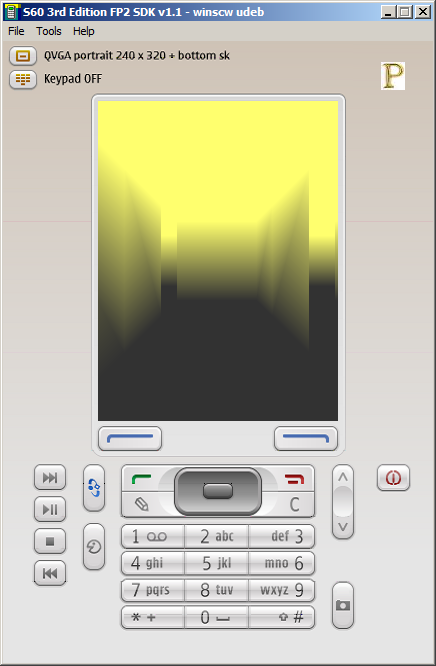
\includegraphics[scale=0.45]{imagenes/ejemplo1.png} \hfill %
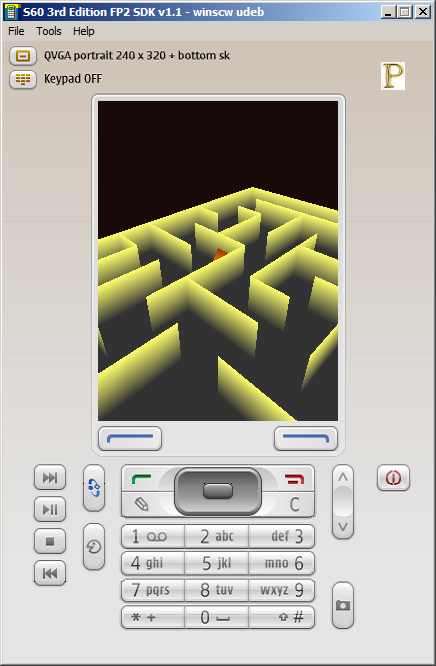
\includegraphics[scale=0.45]{imagenes/ejemplo2.png} \hfill %
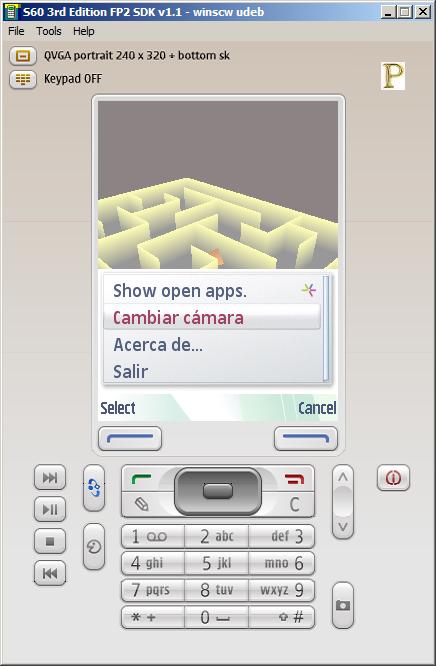
\includegraphics[scale=0.45]{imagenes/ejemplo3.png} %
\caption{Aplicaci�n de ejemplo funcionando sobre el emulador del SDK.}
\label{fig:ejemplos}
\end{figure}

Finalmente, conviene decir que, adem�s de probar este programa en el emulador del SDK, tambi�n se instal� y ejecut� con �xito en un tel�fono m�vil real Nokia 6210 Navigator.

\section{Comparativa con otros SSOO}
La Tabla \ref{table:comparisonOS} muestra una comparativa de los sistemas operativos m�s utilizados en dispositivos m�viles a d�a de hoy. N�tese que la cuota de mercado es una medida que fue tomada en febrero del 2010. El resto de caracter�sticas han sido valoradas en la fecha en la que se escribe el presente documento.

\begin{longtable} {p{1cm} p{3.3cm} | p{3.3cm} | p{3.3cm} |}
\cline{2-4}
\multicolumn{1}{c|}{} & \multicolumn{1}{>{\columncolor[rgb]{0.8, 0.8, 0.8}}c|}{\textbf{Blackberry OS}} & \multicolumn{1}{>{\columncolor[rgb]{0.8, 0.8, 0.8}}c|}{\textbf{iPhone OS}} & \multicolumn{1}{>{\columncolor[rgb]{0.8, 0.8, 0.8}}c|}{\textbf{Android}} \\
\hline
\multicolumn{1}{|>{\columncolor[rgb]{0.8, 0.8, 0.8}}l|}{\textbf{Cuota de mercado\footnotemark[1]{}}} & 20\% & 13\% & 3\% \\
\hline
\multicolumn{1}{|>{\columncolor[rgb]{0.8, 0.8, 0.8}}l|}{\textbf{Plataforma}} & Cerrada & Cerrada & Abierta  \\
\hline
\multicolumn{1}{|>{\columncolor[rgb]{0.8, 0.8, 0.8}}l|}{\textbf{Compa��a}} & RIM & Apple & Google  \\
\hline
\multicolumn{1}{|>{\columncolor[rgb]{0.8, 0.8, 0.8}}l|}{\textbf{Velocidad aplicaciones}} & R�pidas & R�pidas & R�pidas  \\
\hline
\multicolumn{1}{|>{\columncolor[rgb]{0.8, 0.8, 0.8}}l|}{\textbf{Aplicaciones}} & M�s de 3.000 & M�s de 180.000 & Mas de 50.000  \\
\hline
\multicolumn{1}{|>{\columncolor[rgb]{0.8, 0.8, 0.8}}l|}{\textbf{Soporte multi-tarea}} & S� & No & S�  \\
\hline
\multicolumn{1}{|>{\columncolor[rgb]{0.8, 0.8, 0.8}}l|}{\textbf{Soporte multi-touch}} & No & S� & S�  \\
\hline
\multicolumn{1}{|>{\columncolor[rgb]{0.8, 0.8, 0.8}}l|}{\textbf{Navegador Web}} & WebKit & Safari/WebKit & Chrome/WebKit  \\
\hline
\multicolumn{1}{|>{\columncolor[rgb]{0.8, 0.8, 0.8}}r|}{\textbf{Actualizaciones firmware}} & Sync/Patch OTA & Sync/Patch Updates & Al vuelo  \\
\hline
\\[1.5ex]
\multicolumn{1}{c|}{} & \multicolumn{1}{>{\columncolor[rgb]{0.8, 0.8, 0.8}}c|}{\textbf{Palm Web OS}} & \multicolumn{1}{>{\columncolor[rgb]{0.8, 0.8, 0.8}}c|}{\textbf{Symbian OS}} & \multicolumn{1}{>{\columncolor[rgb]{0.8, 0.8, 0.8}}c|}{\textbf{Windows Phone}} \\
\hline
\multicolumn{1}{|>{\columncolor[rgb]{0.8, 0.8, 0.8}}l|}{\textbf{Cuota de mercado\footnotemark{}}} & <3\% & 50\% & 9\% \\
\hline
\multicolumn{1}{|>{\columncolor[rgb]{0.8, 0.8, 0.8}}l|}{\textbf{Plataforma}} & Cerrada & Abierta & Cerrada \\
\hline
\multicolumn{1}{|>{\columncolor[rgb]{0.8, 0.8, 0.8}}l|}{\textbf{Compa��a}} & Palm & Nokia & Microsoft \\
\hline
\multicolumn{1}{|>{\columncolor[rgb]{0.8, 0.8, 0.8}}l|}{\textbf{Velocidad aplicaciones}} & Lentas al arrancar & Muy r�pidas & Depende del terminal \\
\hline
\multicolumn{1}{|>{\columncolor[rgb]{0.8, 0.8, 0.8}}l|}{\textbf{Aplicaciones}} & M�s de 1.400 & M�s de 3.000 & M�s de 18.000 \\
\hline
\multicolumn{1}{|>{\columncolor[rgb]{0.8, 0.8, 0.8}}l|}{\textbf{Soporte multi-tarea}} & S� & S� & Limitada \\
\hline
\multicolumn{1}{|>{\columncolor[rgb]{0.8, 0.8, 0.8}}l|}{\textbf{Soporte multi-touch}} & S� & S� & S� \\
\hline
\multicolumn{1}{|>{\columncolor[rgb]{0.8, 0.8, 0.8}}l|}{\textbf{Navegador Web}} & Chrome/Webkit & Mozilla & Internet Explorer / Trident \\
\hline
\multicolumn{1}{|>{\columncolor[rgb]{0.8, 0.8, 0.8}}r|}{\textbf{Actualizaciones firmware}} & Al vuelo & Sync/Patch OTA & TBA \\
\hline
\caption{Tabla comparativa de sistemas operativos m�viles.}
\label{table:comparisonOS}
\end{longtable}

\footnotetext{Estad�stica para febrero de 2010}

% Secci�n de ap�ndices
% Se a�ade el titulo de "Ap�ndices" al �ndice
%\addcontentsline{toc}{section}{Ap�ndices}

%\input{Apendices.tex}

% A�adimos la bibliografia al �ndice
\clearpage\phantomsection
\addcontentsline{toc}{section}{Referencias}

% Bibliograf�a. En este caso se usa BibTeX
\bibliographystyle{plain}
\pagestyle{plain} 
\bibliography{Bibliografia}

\end{document}
